\chapter{蛇形机器人结构,步态和控制方法}
\label{cha:example}
%\section{图像的插入}
%\subsection{镶嵌在文中的图像}
%\label{sec:Images}
%\begin{wrapfigure}{r}{0.5\linewidth}
%	\centering
%	\includegraphics[width=0.5\textwidth]{image/result/confusion.pdf}
%	\caption{镶嵌在文中的图像}
%	\label{fig:confusion}
%\end{wrapfigure}
%论文主体是毕业论文的主要部分,必须言之成理,论据可靠,严格遵循本学科国际通行的学术规范。在写作上要注意结构合理、层次分明、重点突出,章节标题、公式图表符号必须规范统一。论文主体的内容根据不同学科有不同的特点,一般应包括以下几个方面: (1)毕业论文(设计)总体方案或选题的论证; (2)毕业论文(设计)各部分的设计实现,包括实验数据的获取、数据可行性及有效性的处理与分析、各部分的设计计算等; (3)对研究内容及成果的客观阐述,包括理论依据、创新见解、创造性成果及其改进与实际应用价值等; (4)论文主体的所有数据必须真实可靠,凡引用他人观点、方案、资料、数据等,无论曾否发表,无论是纸质或电子版,均应详加注释。自然科学论文应推理正确、结论清晰;人文和社会学科的论文应把握论点正确、论证充分、论据可靠,恰当运用系统分析和比较研究的方法进行模型或方案设计,注重实证研究和案例分析,根据分析结果提出建议和改进措施等。
%\subsection{单张图像的插入}
%\input{figure/chap03_hole}
%
%\subsection{多张图像的并排插入}
%\label{sub:多张图像的并排插入}
%\input{figure/chap01_example}
%\input{figure/chap04_improve.tex}
%
%\subsection{两列图像的插入}
%\label{sec:complex}
%\input{figure/chap04_voc12_comparison}
%
%\clearpage
%
%\section{表格的插入}
%\label{sec:tables}
%\input{table/chap04_siftflow_result}
%\input{table/chap04_voc_val}
%
%\section{公式}
%\label{sec:formula}
%没有编号的公式
%\begin{align*}
%\begin{split}
%	\label{eq:feedforward}
%	\mybold{z}^{(l)} & = \mybold{W}^{(l)}\mybold{a}^{(l-1)} + \mybold{b}^{(l)} \\
%	\mybold{a}^{(l)} & = f(\mybold{z}^{(l)})
%\end{split}
%\end{align*}
%公式中含有中文
%\begin{align}
%	\begin{split}
%	\mbox{像素准确率} &= \sum_{i=1}^{n_{cl}}n_{ii} / \sum_{i=1}^{n_{cl}}t_i \\
%		\mbox{平均像素准确率} &= \frac{1}{n_{cl}} \sum_{i=1}^{n_{cl}}(n_{ii}/ t_i) \\
%	\mbox{Mean IU} &= \frac{1}{n_{cl}} \sum_{i=1}^{n_{cl}}\frac{n_{ii}}{t_i + \sum_j^{n_{cl}} n_{ji} - n_{ii}}
%	\end{split}
%\end{align}
%公式中含有矩阵
%\begin{equation}
%	\textbf{H} = \begin{bmatrix}
%		I*\mybold{x}_i \\ \textbf{h}
%	\end{bmatrix}
%\end{equation}
%每行后面都有编号的公式
%\begin{align}
%	\frac{\partial}{\partial W_{ij}^{(l)}} J(\mybold{W},\mybold{b};\mybold{x},y) &= \frac{\partial J(\mybold{W},\mybold{b};\mybold{x},y)}{\partial z_i^{(l+1)}}\cdot \frac{\partial z_i^{(l+1)}}{\partial W_{ij}^{(l)}} = \delta_i^{(l+1)}a_j^{(l)} \\
%	\frac{\partial}{\partial b_i^{(l)}} J(\mybold{W},\mybold{b};\mybold{x},y) &= \frac{\partial J(\mybold{W},\mybold{b};\mybold{x},y)}{\partial z_i^{(l+1)}}\cdot \frac{\partial z_i^{(l+1)}}{\partial b_i^{(l)}} = \delta_i^{(l+1)}
%\end{align}
%
%\section{算法流程图}
%\label{sec:algorithm}
%\begin{algorithm}[h]
%\KwIn{$m$个训练样本}
%\lFor{$l=1$ \emph{\KwTo} $n_l$}{
%初始化:$\Delta \mybold{W}^{(l)}=0$,$\Delta \mybold{b}^{(l)}=0$}
%\ForEach{训练样本}{
%	\lFor{$l=1$ \emph{\KwTo} $n_l-1$}{
%	前向传播:$\mybold{z}^{(l+1)}=\mybold{W}^la^l+\mybold{b}^l$,$\mybold{a}^{(l+1)}=f(\mybold{z}^{(l+1)})$}
%	输出误差计算:$\delta^{(n_l)} = \frac{\partial}{\partial \mybold{z}^{(n_l)}} J(\mybold{W},\mybold{b};\mybold{x},y)$\;
%	\lFor{$l=n_l-1$ \emph{\KwTo} $1$}{
%	后向传播:$\delta^{(l)} = \bigl((\mybold{W}^{(l)})^T \delta^{(l+1)}\bigr)f'(\mybold{z}^{(l)})$}
%	\ForAll{层l}{
%		计算梯度:$\nabla_{\mybold{W}^{(l)}}J(\mybold{W},\mybold{b};\mybold{x},y)=\delta^{(l+1)}(\mybold{a}^{(l)})^T$ \\
%		\hspace{60pt}$\nabla_{\mybold{b}^{(l)}}J(\mybold{W},\mybold{b};\mybold{x},y)=\delta^{(l+1)}$\;
%		累加梯度:$\Delta \mybold{W}^{(l)} \leftarrow \Delta \mybold{W}^{(l)} + \nabla_{\mybold{W}^{(l)}}J(\mybold{W},\mybold{b};\mybold{x},y)$; \\
%		\hspace{60pt}$\Delta \mybold{b}^{(l)} \leftarrow \Delta \mybold{b}^{(l)} + \nabla_{\mybold{b}^{(l)}}J(\mybold{W},\mybold{b};\mybold{x},y)$\;
%	}
%}
%\ForAll{层$l$}{
%	更新权重:$\mybold{W}^{(l)} \leftarrow \mybold{W}^{(l)} - \alpha \biggl[\frac 1m \Delta \mybold{W}^{(l)}]$ \\
%	\hspace{60pt} $\mybold{b}^{(l)} \leftarrow \mybold{b}^{(l)} - \alpha \biggl[\frac 1m \Delta \mybold{b}^{(l)}\biggr]$
%}
%\caption{梯度下降算法}
%\label{algo:sgd}
%\end{algorithm}
%
%\section{例子与证明}
%\subsection{例子}
%\begin{eg}
%  这是一个例子, 用以验证特殊环境的字体成功更改为楷体.
%\end{eg}
%
%\begin{proof}
%  1. 大前提
%  2. 小前提
%  结论: 示例结论
%\end{proof}
%
%\section{其他的一些用法}
%\label{sec:font}
%\subsection{子章节编号}
%\label{sec:font:subsection}
%\subsubsection{更小的章节}
%\label{sec:font:subsection:subsub}
%更小的章节编号也是支持的。
%
%\subsection{列表的使用}
%\label{src:font:list}
%
%这是一个无序列表
%\begin{itemize}
%	\item 引用文献\cite{long2015fully}
%	\item 字体{\color{red}{变红}},\textbf{粗体}
%\end{itemize}
%
%这是一个有序列表
%\begin{enumerate}
%	\item 索引前面的章节 \ref{sec:formula}、图像\ref{fig:complex}、表格\ref{tab:siftflow}
%	\item 加脚注\footnote{http://cs231n.github.io/transfer-learning/}
%\end{enumerate}
\section{蛇形机器人模块间的关节连接方式}

\subsection{平行连接}
早期的蛇形机器人关节模块间最常见的连接方式就是平行连接,由Shigeo Hirose研发的第一台蛇形机器人ACM III的连接方式就是平行连接\cite{Endo1999Study}(图\ref{fig:ACM})。ACM III蛇形机器人全场2米,总共由20个索状关节以平行连接的形式构成。在平面中ACM III以蜿蜒曲线步态做运动的速度最高可达40cm/s。
\begin{figure}[h!] % image examples & compare
	\begin{subfigure}{0.5\textwidth}
		\centering
		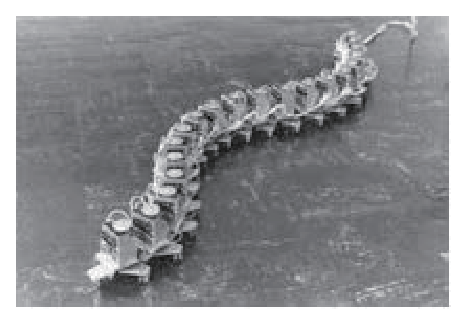
\includegraphics[width=0.6\textwidth,height=0.15\textheight]{figure/chap03/ACMIII.eps}
		\caption{ACM III 样机}
		\label{fig:ACMIII}
	\end{subfigure}
	\begin{subfigure}{0.5\textwidth}
		\centering
		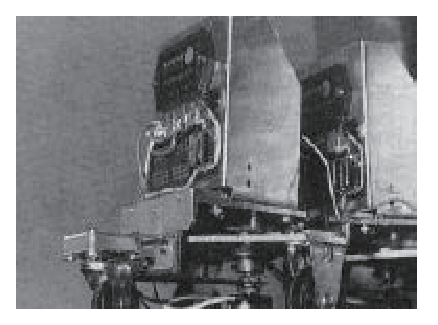
\includegraphics[width=0.6\textwidth,height=0.15\textheight]{figure/chap03/ACMs.eps}
		\caption{ACM III 的局部连接和驱动装置}
		\label{fig:ACMS}
	\end{subfigure}
	\caption{蛇形机器人ACM III}
	\label{fig:ACM}
\end{figure}
采用平行连接连接关节的蛇形机器人的特点为:各个相邻关节的转动都是在一个平面内的,且转动副轴线相互平行且垂直于蛇体的纵轴。对应的最小构成单位为两连杆铰接模型(图\ref{fig:parconnect}),工作空间如图\ref{fig:parspace}所示。
\begin{figure}[h!] % image examples & compare
	\begin{subfigure}{0.5\textwidth}
		\centering
		\includegraphics[width=0.6\textwidth,height=0.15\textheight]{figure/chap03/parellelmod.eps}
		\caption{关节连接}
		\label{fig:parconnect}
	\end{subfigure}
	\begin{subfigure}{0.5\textwidth}
		\centering
		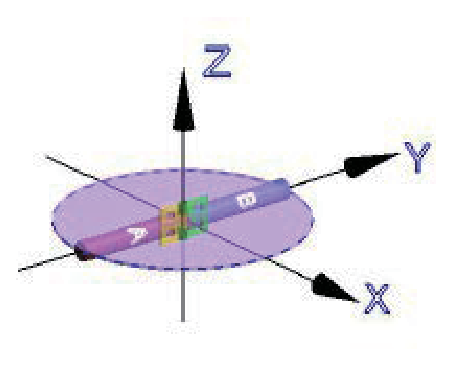
\includegraphics[width=0.6\textwidth,height=0.15\textheight]{figure/chap03/parallelspace.eps}
		\caption{工作空间}
		\label{fig:parspace}
	\end{subfigure}
	\caption{蛇形机器人平行连接结构}
	\label{fig:parallel}
\end{figure}

\subsection{万向连接}
采用万向连接的蛇形机器人的连杆模型的特点为:灵活度高,运动形式多样化。其万向连接的连杆模型为蛇形机器人在三维空间中做灵活,复杂,多样的运动提供了基础。
\begin{wrapfigure}{r}{0.5\linewidth}
	\centering
	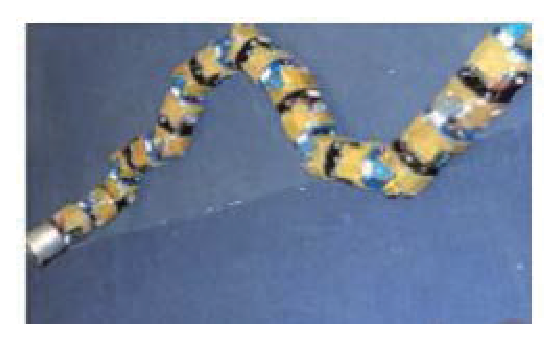
\includegraphics[width=0.4\textwidth]{figure/chap03/scut.eps}
	\caption{华南理工Snakerobot-scut-v5}
	\label{fig:scut}
\end{wrapfigure}图\ref{fig:scut}是由华南理工大学研制的第三代蛇形机器人样机Snakerobot-scut-v5\footnote{http://robotscut.co}。其头部关节采用的是独立的万向关节连接设计,通过在头部安装摄像头和重力感应器后通过特定的算法控制使得蛇形机器人在运动中能够维持头部关节的稳定,通过稳定的蛇形头采集图像,可用于桥梁缆索系统的检测或远程图像的检测提取工作。

基于这种连接的最小单位连接模型为两连杆铰接模型,其连接模型和工作空间如图\ref{fig:all}。
\begin{figure}[h!] % image examples & compare
	\begin{subfigure}{0.5\textwidth}
		\centering
		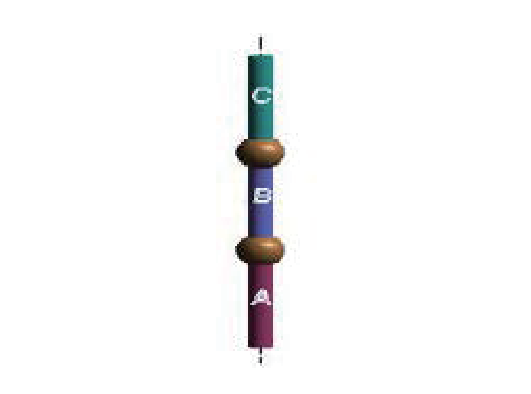
\includegraphics[width=0.6\textwidth,height=0.15\textheight]{figure/chap03/allconnect.eps}
		\caption{关节连接}
		\label{fig:allconnect}
	\end{subfigure}
	\begin{subfigure}{0.5\textwidth}
		\centering
		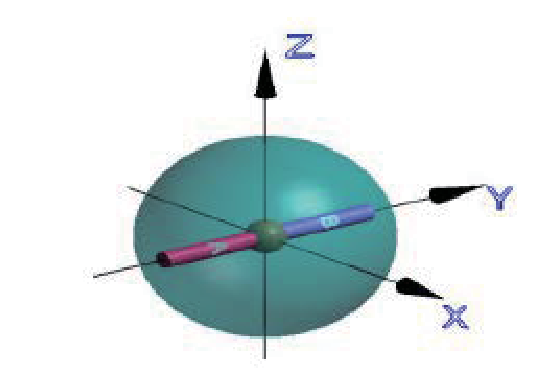
\includegraphics[width=0.6\textwidth,height=0.15\textheight]{figure/chap03/allspace.eps}
		\caption{工作空间}
		\label{fig:allspace}
	\end{subfigure}
	\caption{蛇形机器人万向连接结构}
	\label{fig:all}
\end{figure}


\subsection{正交连接}
为了实现蛇形机器人的三维空间中的运动,Shigeo Hiorse教授的科研团队研发的ARM-R3 蛇形机器人关节间采用正交的方式相连接~\cite{Prautsch1999Control}。采用正交连接的蛇形机器人突破了二维空间运动的桎梏,身体能够进行侧行,翻滚,还能实现内外攀爬的高难度步态。采用关节正交连接设计的蛇形机器人的单元模块和其转动副连接,最小的系统模型为三连杆模型,相邻的转动副呈现垂直的关系。最小系统模型对的关节连接模型如图\ref{fig:orconnect}所示,工作空间如图\ref{fig:orspace}所示。
\begin{figure}[h!] % image examples & compare
	\begin{subfigure}{0.5\textwidth}
		\centering
		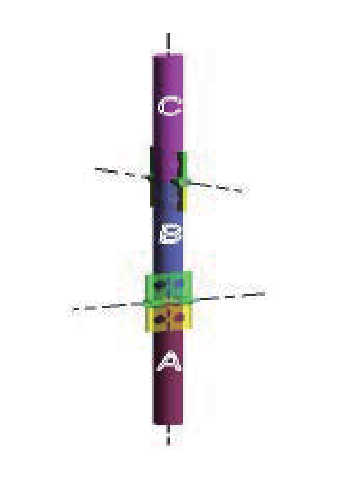
\includegraphics[width=0.35\textwidth,height=0.15\textheight]{figure/chap03/struct.eps}
		\caption{关节连接}
		\label{fig:orconnect}
	\end{subfigure}
	\begin{subfigure}{0.5\textwidth}
		\centering
		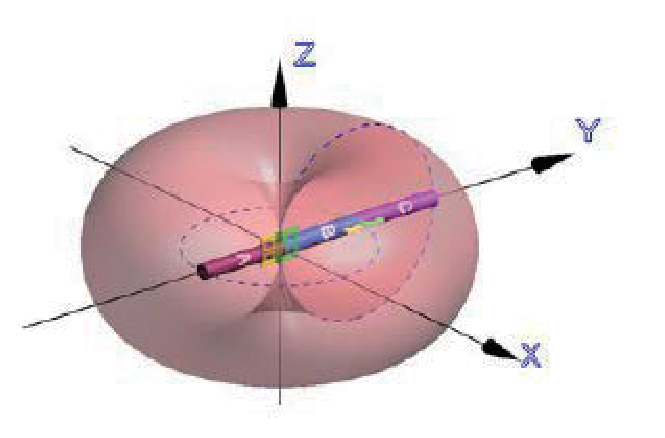
\includegraphics[width=0.9\textwidth,height=0.15\textheight]{figure/chap03/space.eps}
		\caption{工作空间}
		\label{fig:orspace}
	\end{subfigure}
	\caption{蛇形机器人正交连接结构}
	\label{fig:Orthogonal}
\end{figure}
根据正交连接设计的蛇形机器人的实物和仿真下的建模如图\ref{fig:snakeexample}所示。
\begin{figure}[h!] % image examples & compare
	\begin{subfigure}{0.5\textwidth}
		\centering
		\includegraphics[width=0.7\textwidth,height=0.15\textheight]{figure/chap03/realSnake.eps}
		\caption{实物蛇形机器人}
		\label{fig:realSnake}
	\end{subfigure}
	\begin{subfigure}{0.5\textwidth}
		\centering
		\includegraphics[width=0.7\textwidth,height=0.15\textheight]{figure/chap03/simulateSnake.eps}
		\caption{仿真蛇形机器人}
		\label{fig:simulateSnake}
	\end{subfigure}
	\caption{蛇形机器人正交连接设计示例}
	\label{fig:snakeexample}
\end{figure}


\section{蛇形机器人步态}
如今广泛被使用的一个蛇形机器人控制策略是基于Hirose教授提出的正弦运动模型~\cite{HiroseSine},也就是Serpenoid曲线模型,这种运动曲线能够让电机的力矩和摩擦力减小,作为蛇形机器人的运动曲线取得了良好的控制效果,Serpenoid曲线模型如式(\ref{serpenoid})。
\begin{eqnarray}\label{serpenoid}
\left\{
\begin{array}{lr}
x(s)=\int_{0}^{s}\cos \tau d\sigma \\
y(s)=\int_{0}^{s}\sin \tau d\sigma \\
\tau =a\cos(b\sigma )+c\sigma
\end{array}
\right.
\end{eqnarray}

式(\ref{serpenoid})中的a,b,c都是Serpenoid曲线的参数。通过对这几个参数进行修改可以得到不同类型的Serpenoid曲线。$\tau$是波形位置,其改变的速率能够表示曲线运动的速率。$a$,$b$,$c$分别指定了曲线的波动大小,周期以及角速度。由于蛇形机器人的关节模块是独立的刚体,因此通过对曲线公式离散化从而应用到多连杆蛇形机器人的控制中,用蛇形机器人的每个关节去模拟曲线,从而得到每个关节的旋转角度。Serpenoid曲线经过离散化化简之后,各个关节在t时刻的相对的旋转角度即关节角由以下公式给出:
\begin{eqnarray}\label{angledegree}
\phi _{i}(t)=\alpha \sin(\omega t+(i-1)\beta )+\gamma &(i=1,2,...,n-1)
\end{eqnarray}

其中$\alpha$,$\beta$和$\gamma$三个参数决定了蛇形机器人Serpenoid曲线的形状,即运动的步态。$\omega$决定了Serpenoid曲线的传播速率即蛇形机器人运动的速率。


\section{正交设计的蛇形机器人的滚动攀爬步态}
在Hirose教授提出的Serpenoid曲线模型之后,Tesch教授提出了一个蛇形机器人基于正弦运动模型的三维运动参数方程~\cite{ChosetSine}。该参数方程简化了蛇形机器人的控制策略,并实现了用少量控制参数来确定机器人的运动模型。我们实验中采用的是滚动步态~\cite{Enner2013Motion}作为实验中的爬杆步态。滚动步态的正弦运动模型函数如式(\ref{basicRoll})所示:
\begin{eqnarray}\label{basicRoll}
T_i=\left\{
\begin{array}{lr}
A\cdot \sin (\omega \cdot t + i\cdot \varepsilon )&odd\\
A\cdot \sin (\omega \cdot t + i\cdot \varepsilon +  \frac{\pi}{2})&even
\end{array}
\right.
\end{eqnarray}
\begin{figure}[htbp] % image examples & compare
	\begin{subfigure}{0.5\textwidth}
		\centering
		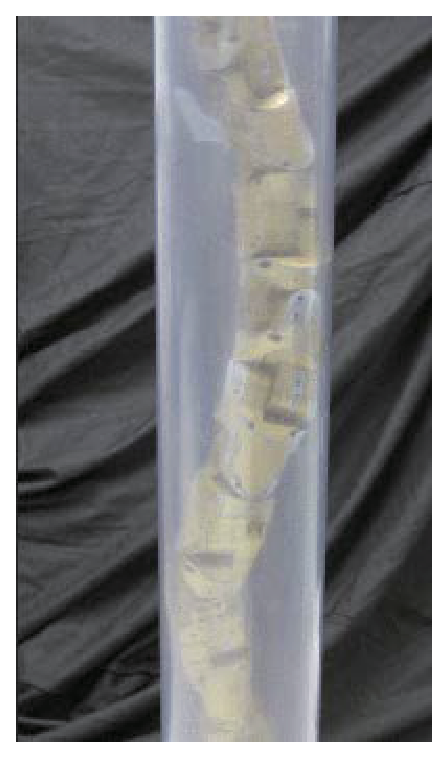
\includegraphics[width=0.5\textwidth]{figure/chap03/pipecrawl.eps}
		\caption{管内攀爬}
		\label{fig:pipecrawl}
	\end{subfigure}
	\begin{subfigure}{0.5\textwidth}
		\centering
		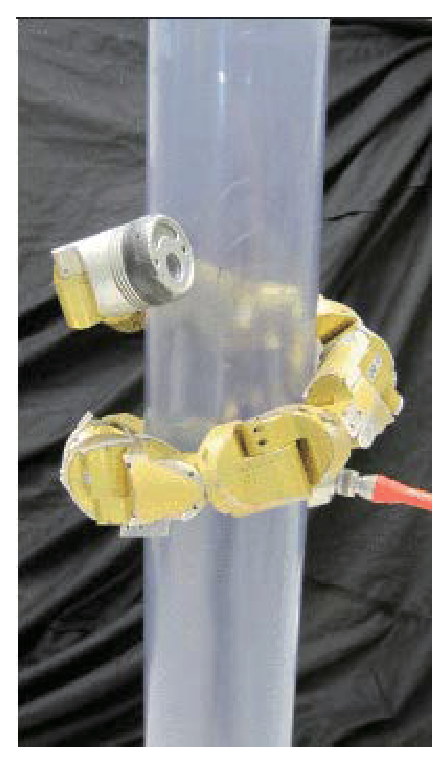
\includegraphics[width=0.5\textwidth]{figure/chap03/poleclimb.eps}
		\caption{管外攀爬}
		\label{fig:poleclimb}
	\end{subfigure}
	\caption{蛇形机器人滚动步态的管道内外攀爬运动}
	\label{fig:polecc}
\end{figure}

通过修改算式\ref{basicRoll}中的幅度参数$A$,相位参数$\varepsilon$和角速度参数$\omega$, 关节的最大可转动角度,机器人的螺旋化程度,蛇形机器人的运动速率会对应地发生改变。与生物蛇不同的是蛇形机器人可以表现出生物蛇无法表现的滚动步态。虽然滚动步态很简单,但是滚动步态确是十分有效的一种运动方式(图\ref{fig:poleclimb})。 通过给予合适的参数,蛇形机器人可以通过滚动步态在地上或者管道内外等环境进行运动。
